\documentclass[german,10pt]{book}     
\usepackage{makeidx}
\usepackage{babel}            % Sprachunterstuetzung
\usepackage{amsmath}          % AMS "Grundpaket"
\usepackage{amssymb,amsfonts,amsthm,amscd} 
\usepackage{mathrsfs}
\usepackage{rotating}
\usepackage{sidecap}
\usepackage{graphicx}
\usepackage{color}
\usepackage{fancybox}
\usepackage{tikz}
\usetikzlibrary{arrows,snakes,backgrounds}
\usepackage{hyperref}
\hypersetup{colorlinks=true,
                    linkcolor=blue,
                    filecolor=magenta,
                    urlcolor=cyan,
                    pdftitle={Overleaf Example},
                    pdfpagemode=FullScreen,}
%\newcommand{\hyperref}[1]{\ref{#1}}
%
\definecolor{Gray}{gray}{0.80}
\DeclareMathSymbol{,}{\mathord}{letters}{"3B}
%
\newcounter{num}
\renewcommand{\thenum}{\arabic{num}}
\newenvironment{anmerkungen}
   {\begin{list}{(\thenum)}{%
   \usecounter{num}%
   \leftmargin0pt
   \itemindent5pt
   \topsep0pt
   \labelwidth0pt}%
   }{\end{list}}
%
\renewcommand{\arraystretch}{1.15}                % in Formeln und Tabellen   
\renewcommand{\baselinestretch}{1.15}                 % 1.15 facher
                                                      % Zeilenabst.
\newcommand{\Anmerkung}[1]{{\begin{footnotesize}#1 \end{footnotesize}}\\[0.2cm]}
\newcommand{\comment}[1]{}
\setlength{\parindent}{0em}           % Nicht einruecken am Anfang der Zeile 

\setlength{\textwidth}{15.4cm}
\setlength{\textheight}{23.0cm}
\setlength{\oddsidemargin}{1.0mm} 
\setlength{\evensidemargin}{-6.5mm}
\setlength{\topmargin}{-10mm} 
\setlength{\headheight}{0mm}
\newcommand{\identity}{{\bf 1}}
%
\newcommand{\vs}{\vspace{0.3cm}}
\newcommand{\noi}{\noindent}
\newcommand{\leer}{}

\newcommand{\engl}[1]{[\textit{#1}]}
\parindent 1.2cm
\sloppy

             \begin{document}     \setcounter{chapter}{3}

\chapter{Gravitationswellen und Newton'sche N\"aherung}

Ebenfalls kurz ansprechen werde ich die Beschreibung 
von Gravitationswellen, den Newton'schen
Grenzfall sowie das Verhalten
von Drehimpuls bzw.\ Spin im Gravitationsfeld.

\section{Gravitationswellen}
\label{Graviton}

Auch ohne \glqq Materie\grqq\ -- ausgedr\"uckt durch den
Energie-Impuls-Tensor $T_{\mu \nu}$ -- haben die Einstein'schen
Feldgleichungen nicht-triviale L\"osungen.
Eine Klasse von L\"osungen der freien Feldgleichungen bilden die
Gravitationswellen. In diesem Fall interessiert man sich f\"ur 
Metriken, die sich nur wenig von der Metrik der flachen Raum-Zeit --
der Minkowski-Metrik $\eta_{\mu \nu}$ -- unterscheiden. Daher bietet 
sich die Aufspaltung
\begin{equation}        
          g_{\mu \nu} ~=~ \eta_{\mu \nu} + \epsilon h_{\mu \nu}   
\end{equation}
an.\index{Einstein'sche Gleichungen!linearisierte} 
Man interessiert sich nun f\"ur die sogenannten linearisierten
Einstein-Gleichungen\index{Linearisierte Einstein-Gleichungen}, d.h.\
es werden nur Terme in linearer Ordnung in $\epsilon$ ber\"ucksichtigt.

In dieser N\"ahrung ergibt sich f\"ur die 
Christoffel-Symbole:\index{Christoffel-Symbole}
\begin{equation}
     \Gamma^\lambda_{~\mu \nu} =  \frac{1}{2} \eta^{\lambda \kappa}
     \left(  \partial_\mu h_{\kappa \nu} + \partial_\nu h_{\mu \kappa}
      - \partial_\kappa h_{mu \nu} \right) 
\end{equation}
(Dieses Ergebnis ist sogar exakt, wenn man $\eta^{\lambda \kappa}$
durch $g^{\lambda \kappa}$ ersetzt.)
F\"ur den Riemann'schen Kr\"ummungstensor 
erhalten wir:\index{Riemann-Christoffel-Kr\"ummungstensor}
\begin{equation}
  R^\lambda_{~\mu \gamma \nu} = \frac{1}{2} \eta^{\lambda \kappa}
  \left( \partial^2_{\mu \gamma} h_{\kappa \nu} + 
  \partial^2_{\kappa \nu} h_{\mu \gamma} -
  \partial^2_{\mu \nu} h_{\kappa \gamma} -
  \partial^2_{\kappa \gamma} h_{\mu \nu}  \right)  \, .  
\end{equation}
(Hier ergeben die in den Christoffel-Symbolen quadratischen
Terme in der linearen N\"aherung keinen Beitrag.)
Die Verk\"urzung \"uber den mittleren unteren Index mit dem oberen
f\"uhrt auf den Ricci-Tensor:\index{Ricci-Tensor}
\begin{equation}
  R_{\mu \nu} = \frac{1}{2} \eta^{\lambda \kappa}
  \left( \frac{\partial^2 h_{\kappa \nu}}{\partial x^\mu \partial x^\lambda} +
   \frac{\partial^2 h_{\mu \lambda}}{\partial x^\kappa \partial x^\nu} -
   \frac{\partial^2 h_{\mu \nu}}{\partial x^\lambda \partial x^\kappa} -
   \frac{\partial^2 h_{\lambda \kappa}}{\partial x^\mu \partial x^\nu} \right) \, .     
\end{equation}

Wie in Abschnitt \ref{sec_EinsteinGl} gezeigt wurde, muss f\"ur eine 
L\"osung der Einstein'schen Feldgleichungen im Vakuum der Ricci-Tensor 
verschwinden. 
Man erh\"alt so eine lineare Differentialgleichung f\"ur $h_{\mu \nu}$:
\begin{equation} 
     \Box h_{\mu \nu} 
   + \frac{\partial^2 h^\rho_{~\rho}}{\partial x^\mu \partial x^\nu}
   - \frac{\partial^2 h^\rho_{~\mu}}{\partial x^\rho \partial x^\nu}  
   - \frac{\partial^2 h^\rho_{~\nu}}{\partial x^\mu \partial x^\rho}
    ~=~ 0  \;.  
\end{equation}

Eine infinitesimale Koordinatentransformation
\begin{equation}
        y^\mu = x^\mu + \epsilon f^\mu(x) \hspace{0.6cm}
        {\rm bzw.} \hspace{0.6cm}
       {\rm d} y^\mu = {\rm d}x^\mu + \epsilon \frac{\partial f^\mu(x)}{\partial x^\nu}{\rm d}x^\nu          
\end{equation}
soll die Metrik nat\"urlich nicht \"andern, d.h. 
\begin{equation}
             \hat{g}_{\mu \nu} {\rm d}y^\mu\, {\rm d}y^\nu =
             g_{\mu \nu} {\rm d}x^\mu\, {\rm d}x^\nu  \, .
\end{equation}              
Die Funktion $h_{\mu \nu}$ transformiert sich in diesem Fall
wie\index{Eichtransformation}
\begin{equation}
     \hat{h}_{\mu \nu} ~=~ h_{\mu \nu} 
    + \frac{\partial f^\mu}{\partial x^\nu}
    + \frac{\partial f^\nu}{\partial x^\mu} \, .  
\end{equation}
Die Funktionen $f^\mu(x)$ sind dabei (im physikalischen Sinne) 
beliebig, und die obige Gleichung beschreibt die Auswirkung 
einer solchen {\em Eichtransformation} auf die Funktion
$h_{\mu \nu}$. \"Ahnlich wie in der
Elektrodynamik k\"onnen wir also eine Eichung w\"ahlen, f\"ur die die
Feldgleichungen eine besonders einfache Form annehmen. Hier w\"ahlt
man \"ublicherweise\index{Eichung}
\begin{equation}
     2 \frac{\partial h^\mu_{~\nu}}{\partial x^\mu}=
         \frac{\partial h^\mu_{~\mu}}{\partial x^\nu}   \;.   
\end{equation}
Durch eine geeignete Wahl von $f_\mu$ lassen sich diese vier Bedingungen
immer erf\"ullen. In dieser Eichung lauten die linearisierten
freien Feldgleichungen:
\begin{equation}
\label{eq_Boxh}
      \Box h_{\mu \nu} ~=~ 0  \;.      
\end{equation}
Dies ist eine gew\"ohnliche Wellengleichung f\"ur die Komponenten 
$h_{\mu \nu}$. Die Eichbedingung f\"uhrt allerdings zu Einschr\"ankungen
zwischen den verschiedenen Komponenten. 

Auch wenn es noch keine zufriedenstellende Quantentheorie der 
Gravitation gibt, so kann man doch vermuten, dass im Grenzfall
kleiner Raum-Zeit-Fluktuationen die Quantentheorie der Gravitation durch
eine quantisierte Form obiger Wellengleichung gegeben ist. Die
zugeh\"origen Teilchen bezeichnet man als Gravitonen.\index{Graviton}
Als Quantenzahlen zum Eigendrehimpuls $h\hbar$ der Gravitonen treten 
zun\"achst
die Werte $h=0,\pm 1,\pm 2$ auf, was Gravitonen als Spin-2-Teilchen
kennzeichnet. Die Helizit\"aten zu $h=0$ und $h=\pm 1$ gibt es jedoch
nicht (\"ahnlich, wie es auch die Helizit\"at $m=0$ f\"ur
das Photon als Spin-1-Teilchen nicht gibt -- da das Photon keine
Masse hat, gibt es auch keine transversalen Freiheitsgrade). 
Lediglich die Helizit\"aten $h=\pm 2$ entsprechen daher der physikalischen
Polarisation einer Gravitationswelle bzw.\ dem Zustand eines Gravitons
(vgl.\ \cite{Fliessbach}, Kap.~29 und 38).

Man versucht heute mit Hilfe von Laserinterferenzexperimenten
(im Wesentlichen riesige Michelson-Morley-Interferometer) 
Gravitationswellen nachzuweisen. Bisher ist ein direkter Nachweis
noch nicht gegl\"uckt, allerdings gibt es indirekte Hinweise auf
Gravitationswellen:\index{PSR 1913+16} 
An Doppelpulsarsystemen (das bekannteste
ist das System PSR 1913+16) beobachtet man \"uber die Jahre
hinweg eine Verk\"urzung der Umlaufzeiten (Abb.\ \ref{fig_PSR}). 
Diese beruht auf
einem Energieverlust, der nach der ART berechnet werden kann
und im Wesentlichen in einer Abstrahlung von Gravitationswellen
besteht.

\begin{SCfigure}[1.5][htb]
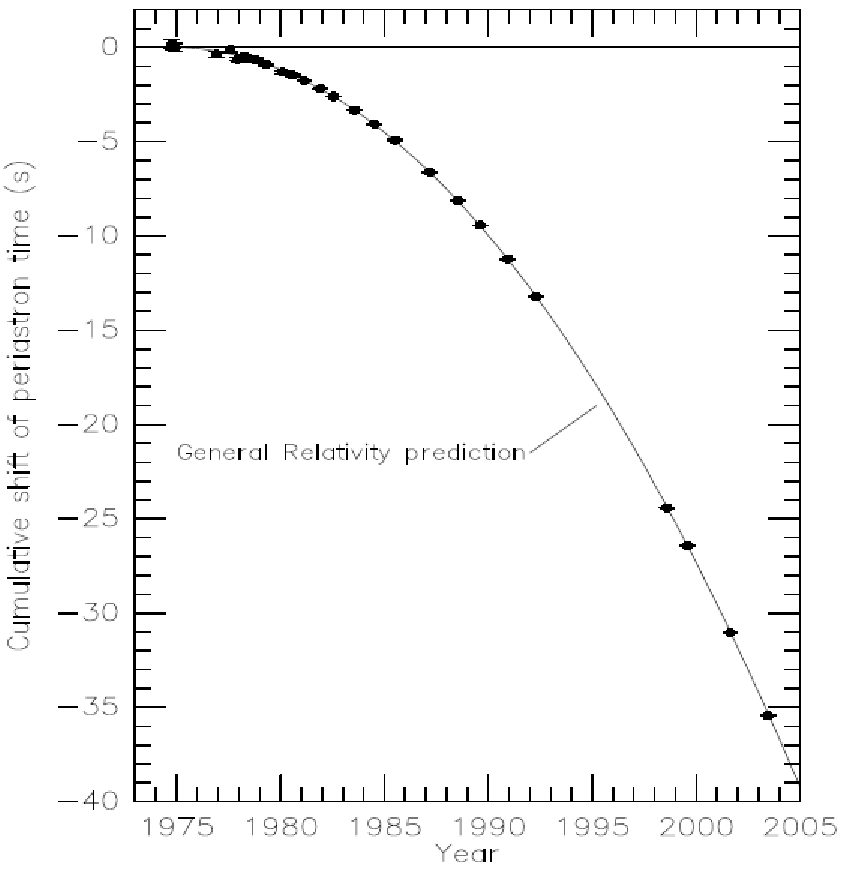
\includegraphics[width=0.5\linewidth, height=0.5\linewidth,%
trim=0 0 0 0,clip]{./Bilder_ART/PSR1913}
\caption{\label{fig_PSR}%
Periodenverk\"urzung des Periastrons (der Punkt, bei dem ein
Stern eines Doppelstern-Systems seinem Partner am
n\"achsten ist) bei dem Doppelstern-System PSR 1913+16.
Die Verk\"urzung beruht im Wesentlichen auf einer
Abstrahlung von Gravitationswellen. (Aus \cite{Weisberg})}
\end{SCfigure}

\section{Die Newton'sche N\"aherung}
\label{sec_NewtonGrenzfall}

Die Geod\"atengleichung (\ref{geodaete}) entspricht
der Bewegungsgleichung f\"ur ein Teilchen unter
dem Einfluss des Gravitationsfeldes. In der Newton'schen
N\"aherung\index{Newton'sche N\"aherung der ART} 
sollte diese Gleichung somit in
\begin{equation}
\label{eq_classV}
      \frac{{\rm d}^2\vec{x}(t)}{{\rm d}t^2} = - \vec{\nabla} \phi(x)
\end{equation}
\"ubergehen, wobei 
\begin{equation}
        \phi(x) = - G \frac{M}{|\vec{x}|}
\end{equation}
das Gravitationspotential eines Massepunktes 
bzw.\ Zentralkraftfelds (dividiert durch die Probemasse) ist. 
F\"ur den Minkowski-Raum verschwinden die
Christoffel-Symbole und man erh\"alt die freie
Bewegungsgleichung. Also muss f\"ur die
Newton'sche N\"aherung eine nicht-triviale
Metrik angenommen werden.

Wenn wir den Grenzfall $v \ll c$ oder
\begin{equation}
      \frac{{\rm d}x^i}{{\rm d}\tau} \ll       \frac{{\rm d}x^0}{{\rm d}\tau} =c \frac{{\rm d}t}{{\rm d}\tau}
\end{equation}
betrachten (das bedeutet, die Vierergeschwindigkeit hat
praktisch nur eine Zeitkomponente), folgt f\"ur die
Beschleunigung:
\begin{equation}
      \frac{{\rm d}^2 x^\mu}{{\rm d} \tau^2} = - \Gamma^\mu_{\nu \lambda}
      \frac{{\rm d}x^\nu}{{\rm d}\tau}\frac{{\rm d}x^\lambda}{{\rm d}\tau}
      \approx - \Gamma^\mu_{00} \left( \frac{{\rm d}x^0}{{\rm d}\tau} \right)^2 \, .
\end{equation}
Au\ss erdem sind wir an statischen L\"osungen interessiert,
bei denen die Metrik keine explizite Zeitabh\"angigkeit hat.
In diesem Fall ist $\Gamma^0_{~00}=0$ und
$\Gamma^k_{00}=\frac{1}{2} \partial^k h_{00}$. Das bedeutet,
in unserer N\"aherung ist
\begin{equation}
      \frac{{\rm d}^2 x^0}{{\rm d} \tau^2} = 0  ~~~ 
      {\rm bzw.} ~~       \frac{{\rm d} x^0}{{\rm d} \tau} = c \frac{{\rm d}t}{{\rm d} \tau} = c  \, .  
\end{equation}
Weiterhin folgt 
\begin{equation}
      \frac{{\rm d}^2 x^k}{{\rm d} \tau^2} 
         =  \frac{{\rm d}^2 x^k}{{\rm d} t^2}       
          = - \frac{1}{2} \frac{\partial h_{00}}{\partial x_k} c^2 
 \end{equation}
oder
\begin{equation}
      \frac{{\rm d}^2 \vec{x}}{{\rm d} t^2} =  \frac{1}{2} \vec{\nabla} h_{00} c^2 \, . 
 \end{equation}
Ein Vergleich mit Gl.\ \ref{eq_classV} gibt uns
\begin{equation}
      h_{00} = - \frac{2\phi}{c^2}  ~~~ {\rm oder} 
                 ~~~ g_{00} = 1 -  \frac{2\phi}{c^2} = 1 -  \frac{2GM}{c^2 r}    \, .
\end{equation}
Damit die Einstein'sche ART im Grenzfall kleiner Geschwindigkeiten
und kleiner statischer Variationen der Metrik (d.h.\ f\"ur gro\ss e
Abst\"ande von einer Massenkonzentration) mit der 
Newton'schen Theorie \"ubereinstimmt, muss in diesem Grenzfall
die Komponente $g_{00}$ der Metrik die Form
\begin{equation}
\label{eq_gnnNewton}
      g_{00} = 1 - \frac{2 G M}{c^2 r} 
\end{equation}
haben. Der Parameter $M$ hat die Interpretation der
Newton'schen Masse. \"Uber die anderen Komponenten der
Metrik k\"onnen wir nichts aussagen. Insbesondere k\"onnen
wir nicht annehmen, dass diese in irgendeinem Sinne klein
im Vergleich zu $g_{00}$ sind. Zur Bewegungsgleichung
tragen sie in dem Grenzfall $v^i \ll c$ nicht bei. 

Nahe der Erdoberfl\"ache k\"onnen wir n\"aherungsweise
$\phi = g h$ setzen ($h$ parametrisiert die H\"ohe \"uber
dem Erdboden) und erhalten
\begin{equation}
      g_{00} = 1 - \frac{2 g h }{c^2} \, .
\end{equation}


\section{Gravity B Probe}

Am 20.\ April 2004 wurde mit einer Rakete ein Satellit 
in die Erdumlaufbahn gebracht, dessen Ziel die
Messung der Raumkr\"ummung in der N\"ahe der
Erde war.\index{Gravity B-Probe} 
Das als \glqq Gravity B Probe\grqq\ bekannte 
Experiment
wurden in der Zeit bis Ende 2005 durchgef\"uhrt, die
Auswertung der Daten dauerte mehrere Jahre.
Zur Ausmessung der Raumkr\"ummung bediente man
sich mehrerer hoch empfindlicher Gyroskope. 

Die Idee des Experiments beruhte darauf, dass der
Drehimpuls ein Vektor ist, der -- sofern andere Einfl\"usse
als die Gravitation ausgeschaltet werden k\"onnen -- 
entlang einer Weltlinie parallel verschoben wird. 
Den 4-Vektor $s^\mu$ erh\"alt man aus der Forderung, dass
der Vektor im Bezugssystem des Gyroskopes
durch $(0,s^i)$ (eine verschwindende Zeitkomponente
und die drei r\"aumlichen Komponenten des Drehimpulses)
gegeben ist.  
Die Pr\"azession\index{Pr\"azession im Gravitationsfeld} 
im Gravitationsfeld erfolgt daher nach der
Gleichung
\begin{equation}
   \frac{{\rm d}s^\mu}{{\rm d}\tau} = - \Gamma^\mu_{\; \nu \lambda}
         u^\nu s^\lambda  \, ,
\end{equation}
wobei $u^\nu(\tau)$ die Komponenten des Tangentialvektors
(in der Eigenzeitparametrisierung) an die Bahnkurve der Verschiebung sind. 
Damit kann man aus einer Rotation der Drehimpulsachse
auf bestimmte Komponenten der Metrik schlie\ss en.

Gravity B Probe sollte zwei Effekte der Raumkr\"ummung
messen:
\begin{enumerate}
\item
Die Raumkr\"ummung durch die Masse der Erde, wie sie
sich beispielsweise aus einer Schwarzschild-Metrik
(siehe n\"achstes Kapitel) f\"ur gro\ss e Abst\"ande vom
Horizont ergibt. Der zu erwartende Effekt aufgrund dieses
Einflusses war pro Jahr rund 6600 Millibogensekunden, 
um den die Drehachse verschoben wird.
\item
Den so genannten {\em Lense-Thirring-Effekt},
wonach\index{Lense-Thirring-Effekt} 
die Raumzeit in der Umgung eines
rotierenden K\"orpers von diesem \glqq mitgezogen\grqq\
wird, was zu einer schwachen Verdrillung der
Raumzeit in der Umgebung eines rotierenden
K\"orpers f\"uhrt. Man kann diesen Effekt z.B.\
aus der Kerr-L\"osung (siehe ebenfalls n\"achstes
Kapitel) f\"ur ein rotierendes
Schwarzes Loch in gro\ss em Abstand erhalten.
Hier betrug der zu erwartende Effekt
rund 40 Millibogensekunden pro Jahr.
\end{enumerate}

Insbesondere der Lense-Thirring-Effekt ist in 
der Umgebung der Erde winzig und erforderte
eine sehr gro\ss e Pr\"azission sowohl bei den
Gyroskopen als auch bei den Ger\"aten zur
Messung der Rotation der Drehimpulsachsen.
Trotzdem konnte der Effekt mit rund 1\% 
Genauigkeit nachgewiesen werden. 

\begin{thebibliography}{99}
%\addcontentsline{toc}{chapter}{Literaturangaben}
%\bibitem{Aichelburg} Peter C.\ Aichelburg (Hrsg.); {\it Zeit im 
%       Wandel der Zeit}; Verlag Vieweg, Braunschweig, Wiesbaden, 1988.
%\bibitem{Barbour3} {\it Mach's Principle -- From Newton's Bucket to
%        Quantum Gravity}; Julian Barbour \& Herbert Pfister (Hrsg.);
%        Birkh\"auser, Boston, Basel, Berlin, 1995.       
%\bibitem{Bekenstein} Jacob D.\ Bekenstein, \textit{Black holes
%          and entropy}, Phys.\ Rev.\ D\,7 (1973) 2333--2346.        
%\bibitem{Bell} John Bell;  {\em Speakable and Unspeakable in 
%        Quantum Physics}, 2.\ edition, Cambridge University Press (2004).       
%\bibitem{Born} Max Born; {\it Optik}; Springer-Verlag, Berlin, Heidelberg,
%        1972.
%\bibitem{Britannica} Encyclopaedia Britannica; 15.th edition, 1988.
%\bibitem{Descartes} Ren\'e Descartes; {\it Die Prinzipien der
%        Philosophie}; Felix Meiner Verlag, Hamburg, 1992; \"ubersetzt
%        von Artur Buchenau.
%\bibitem{EDM} Encyclopaedic Dictionary of Mathematics; Second Edition,
%        MIT Press, 1987.
%\bibitem{Einstein1} Albert Einstein; {\it Zur Elektrodynamik bewegter 
%        K\"orper}; Annalen der Physik, Leipzig, 17 (1905) 891. 
%\bibitem{Einstein2} Albert Einstein; {\it Ist die Tr\"agheit eines
%        K\"orpers von seinem Energieinhalt abh\"angig?} (Ann.\ Phys., 
%        Leipzig, 18 (1905) 639.
%\bibitem{Einstein3} Albert Einstein; {\it Aus meinen sp\"aten Jahren};
%         Ullstein Sachbuch, Verlag Ullstein, Frankfurt, Berlin, 1993.                 
%\bibitem{Einstein4} Albert Einstein; {\it Prinzipielles zur allgemeinen
%        Relativit\"atstheorie}; Annalen der Physik 55 (1918) 241.
%\bibitem{Einstein5} Albert Einstein; {\it \"Uber den Einflu\ss\ der
%        Schwerkraft auf die Ausbreitung des Lichtes}; Annalen der
%        Physik 35 (1911) 898.                 
%\bibitem{Feynman} Richard Feynman; {\it The Character of Physical Law};
%        The MIT Press, 1987.        
%\bibitem{Fierz} Markus Fierz; {\it \"Uber den Ursprung und die Bedeutung
%        der Lehre Isaac Newtons vom absoluten Raum}; Gesnerus, 
%        11.\ Jahrgang (1954), S.\,62--120.
%\bibitem{Fliessbach} Torsten Flie\ss bach; {\it Allgemeine 
%        Relativit\"atstheorie}; BI-Wissenschaftsverlag, Mannheim, Wien
%        Z\"urich, 1990. 
%\bibitem{Galilei} Galilei; {\it Dialog \"uber die beiden haupts\"achlichen
%        Weltsysteme, das ptolem\"aische und das kopernikanische}; 
%        Teubner Stuttgart, 1982; aus dem Italienischen \"ubersetzt von
%        Emil Strauss.   
%  \bibitem{Hawking} Stephen W.\ Hawking, \textit{Particle Creation by
%            black holes}, Comm.\ Math.\ Phys.\ 43 (1976) 199--220.      
%\bibitem{Helmholtz2} Hermann von Helmholtz; {\em \"Uber Wirbelbewegungen,
%        \"Uber Fl\"ussigkeitsbewegungen}, 1858; in Ostwalds Klassiker der 
%       exakten Wissenschaften Bd.\ 1; Verlag Harri Deutsch, Frankfurt, 
%       1996.                   
%\bibitem{Lamb} G.L.\ Lamb, Jr.; {\it Elements of Soliton Theory}; 
%         Pure \& Applied Mathematics, John Wiley \& Sons, 1980. 
%\bibitem{Laue} Max von Laue; {\it Geschichte der Physik}; 
%         Universit\"ats-Verlag Bonn, 1947.
%\bibitem{Lorentz} Hendrik Antoon Lorentz; {\it Electromagnetic phenomena 
 %        in a system moving with any velocity smaller than that of light}; 
%         Proc.\ Acad.\ Sci., Amsterdam, 6 [1904], S.\ 809.
%\bibitem{Mach} Ernst Mach; {\it Die Mechanik in ihrer Entwicklung
%      historisch kritisch dargestellt}; Akademie Verlag, Berlin, 1988.       
%\bibitem{Mainzer} Klaus Mainzer; {\it Philosophie und Geschichte von
%         Raum und Zeit}; in {\it Philosophie und Physik der Raum-Zeit};
%         J\"urgen Audretsch und Klaus Mainzer (Hrsg.); 
%         BI-Wissenschaftsverlag, 1994. 
%\bibitem{Microscope} Touboul, Pierre, et al. (MICROSCOPE Collaboration); \textit{MICROSCOPE Mission:
%         Final Results of the Test of the Equivalence Principle}; Phys.\ Rev.\ Lett.\ \textbf{129} (2022) 121102.
%\bibitem{Misner} C.W.\ Misner, K.S.\ Thorne, J.A.\ Wheeler; 
%        {\it Gravitation}; W.H.\ Freeman and Company, San Francisco,  1973.
%\bibitem{Mittelstaedt} Peter Mittelstaedt; {\it Der Zeitbegriff in der
%        Physik}; BI-Wissenschaftsverlag, 1989.        
%\bibitem{Mittelstaedt2} Peter Mittelstaedt; {\it Philosophische Probleme
%        der modernen Physik}; BI-Wissenschaftsverlag, 1989.        
%\bibitem{Newton}
%   Isaac Newton; {\it Mathematische Grundlagen der Naturphilosophie}; 
%   \"ubersetzt von Ed Dellian; Felix Meiner Verlag, 1988. 
%\bibitem{Newton2} Isaac Newton; {\it \"Uber die Gravitation...};
%       Klostermann Texte Philosophie; Vittorio Klostermann, Frankfurt,
%      1988; \"ubersetzt von Gernot B\"ohme.
%\bibitem{Newton3} Isaac Newton; {\it Optik oder Abhandlung \"uber
%      Spiegelungen, Brechungen, Beugungen und Farben des Lichts};
%      I., II.\ und III.\ Buch (1704); aus dem Englischen \"ubersetzt
%      von W.\ Abendroth; Ostwalds Klassiker der exakten Wissenschaften,
%      Verlag Harri Deutsch 1998.   
%\bibitem{Neumann} Carl Neumann; {\it \"Uber die Principien der
%         Galilei-Newtonschen Theorie}; Akademische Antrittsvorlesung,
%         gehalten in der Aula der Universit\"at Leipzig am 3.\ Nov.\
%         1869; Teubner (Leipzig) 1870.         
%\bibitem{Pauli} Wolfgang Pauli; {\it Theory of Relativity}; Dover
%      Publications, New York, 1981.      
%\bibitem{Poincare} Jules Henri Poincar\'e; {\it Sur la dynamique de 
%     l'\'electron}, C.R.\ Acad.\ Sci., Paris, 140 (1905) S.~1504; und 
%      Rendiconti del Circolo Matematico di Palermo, Bd.~21 (1906) S.~129.
%\bibitem{Reichenbach1} Hans Reichenbach; {\em Philosophie der 
%       Raum-Zeit-Lehre}; Hans Reichenbach - Gesammelte Werke Bd.\ 2;
%       Vieweg-Verlag, Braunschweig; 1977.
%\bibitem{Reichenbach2} Hans Reichenbach; {\em Axiomatik der
%       relativistischen Raum-Zeit-Lehre}; in {\em Die philosophische
%       Bedeutung der Relativit\"atstheorie}; Hans Reichenbach - Gesammelte
%       Werke Bd.\ 3; Vieweg-Verlag, Braunschweig, 1977. 
%\bibitem{Rovelli} Carlo Rovelli, \textit{Quantum Gravity}; Cambridge
%      University Press, 2007.       
%\bibitem{Schlamminger} Schlamminger, Choi, Wagner, Gundlach,
%         Adelberger; {\em Test of the Equivalence Principle using a
%         rotating torsion balance}; Phys.\ Rev.\ Lett.\ {\bf 100} (2008)
%         041101.     
%\bibitem{Sexl} Roman U.\ Sexl, Helmuth K.\ Urbantke; {\it Relativit\"at,
%      Gruppen, Teilchen}; Springer-Verlag, Wien, New York, 1992.
%\bibitem{Simonyi}
%       K\'aroly Simonyi; {\it Kulturgeschichte der Physik}; Verlag
%       Harri Deutsch, Thun, Frankfurt am Main, 1990.
%\bibitem{Weisberg} Weisberg, J.M., Taylor, J.H.; {\em Relativistic Binary Pulsar
%          B1913+16: Thirty Years of Observations and Analysis}; 
%          \verb+arXiv:astro-ph/0407149v1+; 2004. 
%\bibitem{Thomson} James Thomson; {\it On the Law of Inertia; the
%       Principle of Chronometry; and the Principle of Absolute Clinural
%       Rest, and of Absolute Rotation}; Proc.\ Roy.\ Soc.\ (Edinburgh),
%       Session 1883-84, Vol.\ XII, 568--578.       
%\bibitem{Weizsaecker} Carl Friedrich von Weizs\"acker; {\em Der zweite
%      Hauptsatz und der Unterschied von Vergangenheit und Zukunft};
%      Annalen der Physik 36 (1939) 275--283.       
%\bibitem{Zeh} Zeh, H.D.; {\em The Physical Basis of the Direction of Time},
%      Springer-Verlag, Berlin, 1989.       

%\bibitem{Einstein} Einstein, Albert; {\em ??}, .                   
\end{thebibliography}


\end{document}
